\documentclass{style}
\usepackage[urlcolor=blue]{hyperref}
\usepackage{setspace}
\usepackage{graphicx}
\usepackage{titlesec}
\usepackage{fontspec}
\usepackage{float}
\usepackage{ctex}
\newcommand{\upcite}[1]{\textsuperscript{\textsuperscript{\cite{#1}}}}
\usepackage{fancyhdr}
\titleformat{\section}{\large \heiti}{\chinese{section}、}{0em}{}

% \usepackage[usenames,dvipsnames]{xcolor}

%%
%% Julia definition (c) 2014 Jubobs
%%
\lstdefinelanguage{Julia}%
  {morekeywords={abstract,break,case,catch,const,continue,do,else,elseif,%
      end,export,false,for,function,immutable,import,importall,if,in,%
      macro,module,otherwise,quote,return,switch,true,try,type,typealias,%
      using,while},%
   sensitive=true,%
   alsoother={$},%
   morecomment=[l]\#,%
   morecomment=[n]{\#=}{=\#},%
   morestring=[s]{"}{"},%
   morestring=[m]{'}{'},%
}[keywords,comments,strings]%

\lstset{%
    language        = Julia,
    basicstyle      =\fontspec{Lucida Console},
    stringstyle     =\color{red!45!green!80},
    keywordstyle    =\color{blue!50}\bfseries,
    commentstyle    =\color{red!30!green!50!blue!30},
    frame           =shadowbox,
    framerule       =1pt,
    backgroundcolor =\color{white!20}
}

\begin{document}
\begin{center}
      \LARGE \textbf{对称操作群的导出和马德隆常数的快速计算}\\
      \vspace{0.3em}
      \large 作者:张浪 \quad 学号:1608405066 \\ %姓名,学号
\end{center}
\rule[0.1\baselineskip]{\textwidth}{0.5pt}
\textbf{摘 \ 要}\\
\large
本文通过分析几何空间的对称划分特性,得出几何空间的对称操作和最小对称等分子空间的空间位置变换有着一一对应的关系,而最大围绕几何中心对称等分数即是对称操作数,可以从对称等分的角度导出几何空间的对称操作群的结论;并应用空间的对称特性来实现对NaCl和CsCl等立方晶体的马德隆常数的快速计算。
\\
\\
\textbf{关键词}:对称操作群\quad 对称等分\quad 马德隆常数\\
\rule[0.1\baselineskip]{\textwidth}{0.5pt}
\section*{引言}
大多数晶体在几何外形上都表现出良好的对称性。实际上,无论是在自然界还是在人类社会,无论是个体还是群体,小到微观粒子,大到宏观天体,我们都可以在其中找到各种对称性,比如动物身体结构的几何对称,以及无处不在的电荷对称和磁极对称。可以说,对称性无处不在。对对称性的正确应用不仅可以增加结构和形式上的美感,对于问题的求解也能给出极大的简化效果。

\section{对称操作群的导出} % (fold)
\label{sec:对称操作群的导出}
在本节中,我们将探讨几何空间的对称等分特性和对称操作之间存在的关系,并得出几何空间的对称操作和最小对称等分子空间的空间位置变换一一对应的结论。\\
\indent 在后续论述中,我们将遵循如下两个约定:\\
\indent 1.对几何中心和对称中心这两个名词不进行区分,皆指几何空间的对称中心;\\
\indent 2.原几何中心一词指我们对其进行对称等价划分的原始几何空间的对称中心。
\subsection{定义}
围绕几何中心对称等分,是按照一定的对称特性将一个几何空间围绕着它的几何中心划分为N个全等的子空间,划分后这N个子空间以原几何中心作为共同的顶点。如果单个子空间关于原几何中心依然具有对称性,那么可以将子空间进一步关于原几何中心对称划分,直到子空间关于原几何中心不再具有对称性,这时的子空间称为该几何空间的\bold{最小对称等分子空间},子空间的个数称作该几何空间的\bold{最大围绕几何中心对称等分数}。

\subsection{探索发现} % (fold)
\label{sub:探索发现}
以下通过分析和计算立方空间、正四面体空间和正六角柱空间的最大围绕几何中心对称等分数,探索最大围绕几何中心对称等分数和对称操作数之间存在的关系。
\subsubsection{立方空间}
\label{sub:立方空间}
对于立方体,以其几何中心为原点O,过几何中心垂直于各个面的直线作为坐标轴,建立直角坐标系Oxyz。则此直角坐标系将原立方体对称等分为8个立方子空间,其中每个立方子空间关于原点(原几何中心)依然存在对称性,下面关于原点的对称等分适用于每一个立方子空间。
以全正半轴子空间$Ox_+y_+z_+$为例,设此子空间的长宽高分别为$x_0, y_0, z_0$,并令点$(x_0, y_0, z_0)$为点A,连接体对角线$OA$,过点A作3条坐标轴的垂线,接着连接过原点的3条面对角线,我们将得到6个平面。这6个平面相交于体对角线$OA$,相邻的两个面之间的夹角都为$60^\circ$,刚好把此立方子空间等分为6个全等的四面体子空间,这6个四面体子空间以原点为共同的顶点,单个四面体子空间关于原点不再具有对称性。对于8个立方子空间中的每一个,我们都可以实施这种对称等分。因此,立方空间最多可以围绕其几何中心对称等分为$8\times6=48$个子空间,即立方体空间的最大围绕几何中心对称等分数为48。
\begin{figure}[H]
\begin{minipage}[H]{0.5\linewidth}
\centering
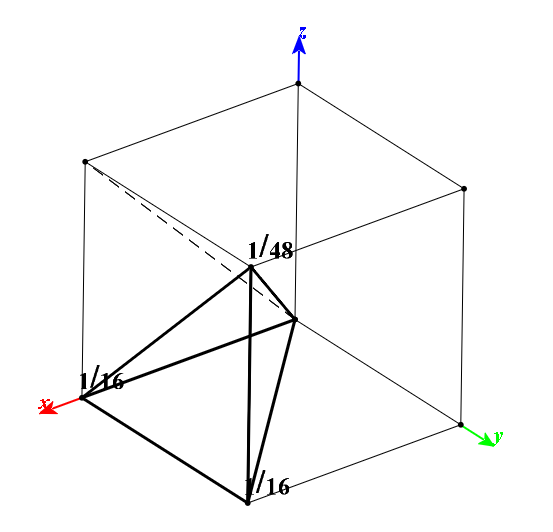
\includegraphics[width=3in]{透视.png}
\caption{立方体最小对称等分子空间透视图}
\label{fig:side:a}
\end{minipage}%
\begin{minipage}[H]{0.5\linewidth}
\centering
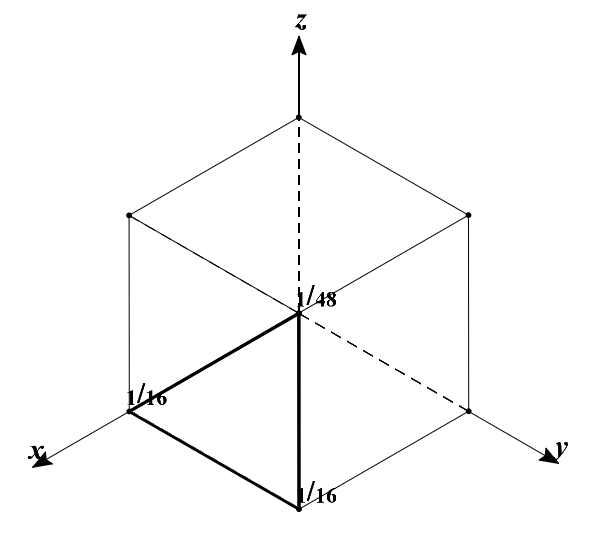
\includegraphics[width=3in]{111.png}
\caption{立方体沿体对角线的投影}
\label{fig:side:b}
\end{minipage}
\end{figure}

\subsubsection{正四面体空间} % (fold)
\label{sub:b_正四面体空间}
对于正四面体空间,设其对称中心为点O,连接点O和正四面体的四个顶点,这些线段同此正四面体的棱组成的平面把这个正四面体对称等分为4个全等的四面体子空间。四面体子空间的底面为正三角形,侧面是3个全等的等腰三角形,关于正四面体的几何中心依然存在对称性。对于每一个四面体子空间,根据正三角形的对称性,我们又可以将之围绕其顶点和底面正三角形中心的连线对称等分为6个全等的四面体子空间,这些四面体子空间关于正四面体的几何中心不再具有对称性。因此,通过一系列对称等分,我们可以把正四面体空间划分为$4\times6=24$个对称等价且不再具对称性的四面体子空间。综上所述,正四面体空间的最大围绕几何中心对称等分数为24。
% subsubsection* b_正四面体空间 (end)

\subsubsection{正六角柱空间} % (fold)
\label{sub:c_正六角柱空间}
通过类似上述的方法,我们可将正六角柱空间关于其几何中心对称等分为$2\times6\times2=24$个全等的以原几何中心为共同顶点且关于原几何中心不再具有对称性的三棱柱子空间。故正六角柱空间的最大围绕几何中心对称等分数为24。
% subsubsection* c_正六角柱空间 (end)
% subsection 探索发现 (end)

\subsection{归纳推理} % (fold)
\label{sub:归纳推理}
立方体、正四面体和正六角柱这3种几何空间的对称操作数分别为48,24,24。以上的分析和计算表明:这3种几何空间的最大围绕几何中心对称等分数与其对称操作数一一对应相等。那么是否所有的空间都具有此种性质呢?下面以立方体为例,对几何空间的对称操作和最小对称等分子空间的空间位置变换一一对应,对称操作数与其最大围绕几何中心对称等分数相等这一结论作简要的演绎证明。其他几何空间也可相应证明。
% subsection 归纳推理 (end)

\subsection{演绎证明} % (fold)
\label{sub:演绎证明}
对于立方体,以几何中心为原点建立的直角坐标系将其划分为8个立方子空间,每个子空间通过一个位置变换的矩阵都可以唯一地变换到另一个子空间,这8种位置变换组成一个位置变换群,群元的乘积依然是群元。而在此位置变换的基础上,立方子空间进一步对称等分得到的四面体子空间之间的6种位置变换又组成一个位置变换群(由于每一种位置变换都唯一地把一个子空间变换到另一个子空间,故$C=BA$表示的连续进行两个变换的变换依然是群元)。设立方子空间关于原立方空间的一个位置变化为$T_1$,最小对称等分子空间关于立方子空间的一个位置变换为$T_2$,显然,由于$T_2$是在$T_1$的基础上进行的,故$T_2T_1$合成的所有位置变换组成了最小对称等分子空间关于原几何中心的位置变换群,一共$8\times6=48$个群元,也即立方空间的对称操作数位数48。\\

实际上,一个几何空间的N个最小对称等分子空间以原空间的几何中心为共同的顶点,形状完全相同,但每个子空间具有独一无二的空间位置。而一个对称操作可唯一地把一个最小对称等分子空间变换到另一个最小对称等分子空间。因此,最小对称等分子空间空间位置的变换和对称操作一一对应,而最大围绕几何中心对称等分数即是对称操作数。
% subsection  (end)
% section 对称操作群的导出 演绎证明(end)

\section{马德隆常数的快速计算} % (fold)
\label{sec:马德隆常数的快速计算}
在计算晶格的马德隆常数时,如若按找普通的方法,计算$N^3$个格点,通常需要$N^3$次计算,而应用晶格的空间对称特性,我们将能够有效地缩减计算量。 这其中的要点在于,如何将空间围着对称中心划分到最小,然后在计算时只对划分后一个子分子空间进行计算。以上的分析告诉我们,在计算NaCl和CsCl等立方晶格的马德隆常数时,只需计算其最小对称等分子空间的系数和,然后乘以48,便可得到真正的马德隆常数,因此我么我们在计算$N^3$个格点时,计算将缩减至$N^3/48$,因而速度是普通的方法的48倍。
同时,考虑到我们的目的是编写程序应用计算机快速计算马德隆常数,因此在编程时,考虑到离子电性的周期性,我们可以通过周期性地变换一个变量的符号来消除对$-1$幂次的重复计算。

综上所述,约化后的立方晶体马德隆常数的计算公式为:
\begin{equation}\label{eqution:fast_madelung}
    \alpha = 48\sum\limits_{i=1}^{N}\sum\limits_{j=1}^{i}\sum\limits_{k=1}^{j}{\frac{C\times(-1)^{i+j+k}}{(i^2+j^2+k^2)^{1/2}}}
\end{equation}
其中C为占比常数,需根据原子在最小对称等分子空间中的位置考虑。\\
\indent a. 对于棱上的原子,C的取值为$\theta/360$,$\theta$为该条棱上两个面的夹角的度数;\\
\indent b. 对于边界面上的原子,C一律取$1/2$;\\
\indent c. 对于空间内部的原子,C取值为1;\\
\indent d. 对于顶点处的3个原子需特殊考虑。\\

下列两张图说明了C的取值特点。\\
\begin{figure}[H]
\begin{minipage}[H]{0.5\linewidth}
\centering
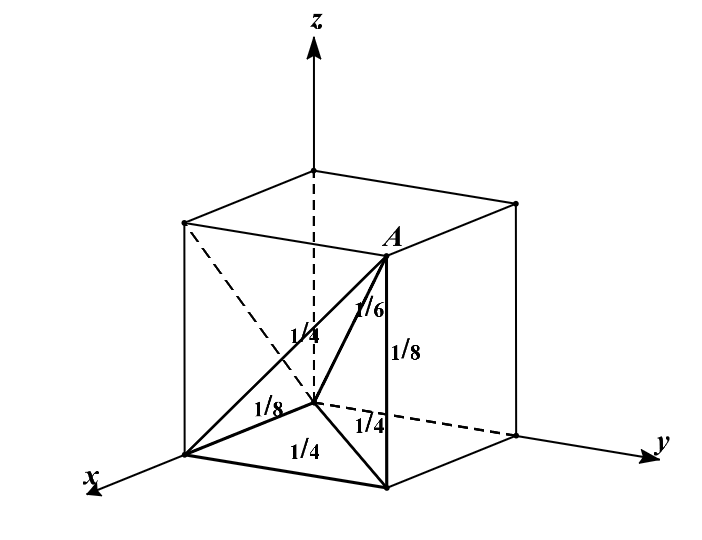
\includegraphics[width=3.2in]{棱上原子.png}
\caption{棱上原子}
\label{fig:side:a}
\end{minipage}%
\begin{minipage}[H]{0.5\linewidth}
\centering
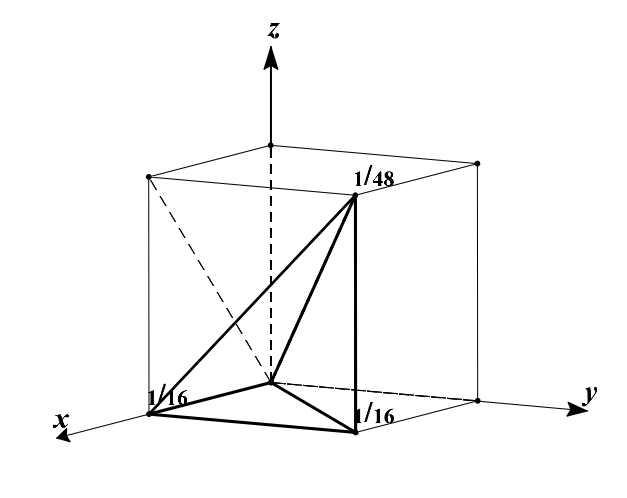
\includegraphics[width=3in]{顶点原子.png}
\caption{顶点原子}
\label{fig:side:b}
\end{minipage}
\end{figure}

\newpage
\indent 根据公式(\ref{eqution:fast_madelung}),并考虑NaCl晶格中正负原子的分布特点,计算NaCl的马德隆常数的伪代码可如下给出:
\begin{center}
\begin{lstlisting}
function NaCl48(N::Int64)
    m1, m2, m3, m4, m5 = 0.0, 0.0, 0.0, 0.0, 0.0
    N = N + (N & 0x1)
    e1, N² = 1.0, N^2
    for n1 = 1:N-1
        e1 = e2 = -e1
        n1² = n1^2
        # 坐标轴上: 1/8
        # 面对角线: 1/4 × 1/√2 = √2/8
        # 体对角线: 1/6 × 1/√3 = √3/18
        m1 += (√2/8 + e1 * (1/8 + √3/18)) / n1
        m4 += 1.0/ √(N² + 2n1²)  #棱: x = N, y = z, 1/4
        m4 += e1 / √(N² + n1²)   #棱: x = N, z = 0, 1/4
        m5 += e1 / √(2N² + n1²)  #棱: x = N, y = N, 1/8
\end{lstlisting}
\end{center}
第一层循环计算了最小对称等分子空间(四面体)棱上的原子,其中通过对变量e1的不断取反,消除了$-1$的$n$次幂的计算,下面亦如是。\\

第二层循环累计边界面上的原子的系数和。
\begin{center}
\begin{lstlisting}
        for n2 = n1+1:N-1
            n2² = n2^2
            AB = n1² + n2²
            e2 = -e2
            e3 = e1 * e2
            # m2累计边界面上的原子,结果只计m2/2
            m2 += e3 / √(AB)       #面: z = 0
            m2 += e3 / √(AB + N²)  #面: x = N
            m2 += e2 / √(AB + n1²) #面: x = y
            m2 += e1 / √(AB + n2²) #面: y = z
\end{lstlisting}
\end{center}

\newpage
第三层循环累计三棱锥空间内部的原子的系数和。
\begin{center}
\begin{lstlisting}
            e3 *= e2
            # m3累计三棱锥空间内部的原子
            for n3 = n2+1:N-1
                e3 = -e3
                m3 += e3 / √(AB + n3^2)
            end
        end
    end
    m3 += m4/4 + m5/8 + (1 + √2/2 + √3/9)/16N
    return -48(m1 + m2/2 + m3)
end
\end{lstlisting}
\end{center}
% section* 马德隆常数的快速计算 (end)

\begin{thebibliography}{9}%宽度9
\bibitem{bib:one} 黄昆、韩汝琦,固体物理学,高等教育出版社,1985年3月
\end{thebibliography}

\appendix
\section*{附录}
快速计算NaCl和CsCl的马德隆常数的完整代码见:
\begin{center}
https://github.com/absop/MadelungConst
\end{center}

\end{document}
